\documentclass[11pt]{article}
\usepackage[margin=1in]{geometry}
\usepackage{longtable}
\usepackage{booktabs}
\usepackage{array}
\usepackage{enumitem}
\usepackage{hyperref}
\usepackage{xurl}
\usepackage{tikz}
\usetikzlibrary{arrows.meta, positioning, shapes.geometric}

\title{Phase-2 Deliverable: Adapter Contract}
\author{SIT Engine Phase-2}
\date{\today}

\begin{document}
\maketitle

% Improve longtable wrapping/spacing for long code paths.
\setlength{\tabcolsep}{4pt}
\renewcommand{\arraystretch}{1.15}
\newcommand{\codepath}[1]{\path{#1}}

\section{Technical Description}
The Adapter Contract is the formal boundary between platform-specific trace parsing and platform-agnostic SIT analytics. Its purpose is to prevent semantic leakage by forcing all source traces to be normalized before entering engine/window logic.

In Phase-2 architecture, this deliverable is the stability layer that allows the same engine to process traces from CPU raw logs, Spike, and gem5 through one canonical ingest schema.

\subsection*{Done-When Criterion}
\textbf{Done when all adapters conform without semantic leakage.}
\begin{itemize}[leftmargin=*]
  \item Conform: each adapter emits valid normalized state/residency intervals.
  \item No semantic leakage: adapter layer does not implement SIT window math, summary policy, or export contract logic.
\end{itemize}

\section{Implementation Fulfillment}
Repository paths that fulfill the contract:

\begin{longtable}{@{}>{\raggedright\arraybackslash}p{0.36\textwidth} >{\raggedright\arraybackslash}p{0.60\textwidth}@{}}
\toprule
\textbf{Code Path} & \textbf{Fulfillment Responsibility} \\
\midrule
\endhead
\codepath{Phase-2/ingest/ingest_api.py} &
Defines formal interface and validators:
\texttt{TraceAdapter} protocol (\texttt{load\_state\_intervals()}, \texttt{load\_residency\_intervals()}),
\texttt{validate\_state\_df()}, \texttt{validate\_resid\_df()},
state set \{\texttt{active}, \texttt{stall}, \texttt{idle}\}, and interval sanity (\texttt{end\_us > start\_us}). \\
\addlinespace
\codepath{Phase-2/adapters/baseline_adapter.py} &
Implements contract-facing adapter behavior for normalized CSV and delegated raw parsing. Calls validators before returning data. \\
\addlinespace
\codepath{Phase-2/adapters/cpu_adapter.py} &
Parses raw workload events to normalized state and residency dataframes (\texttt{to\_state\_dataframe()}, \texttt{to\_residency\_dataframe()}). \\
\addlinespace
\codepath{Phase-2/adapters/spike_adapter.py} &
Normalizes Spike commit logs into contract outputs via
\texttt{build\_state\_intervals()}, \texttt{build\_residency\_intervals()}, and validator enforcement. \\
\addlinespace
\codepath{Phase-2/adapters/gem5_adapter.py} &
Normalizes gem5 Exec traces into the same contract fields with marker-aware residency and state classification. \\
\addlinespace
\codepath{Phase-2/adapters/adapter_template.py} &
Template implementation that encodes the required contract pattern for new adapters. \\
\addlinespace
\codepath{Phase-2/cli.py}, \codepath{Phase-2/riscvbench.py} &
Operational integration points consuming adapter outputs through the normalized pipeline. \\
\addlinespace
\codepath{Phase-2/run_cross_target_suite.py}, \codepath{Phase-2/tests/run_golden_suite.py} &
Executable conformance checks validating that adapter outputs produce expected downstream artifacts and invariant behavior. \\
\bottomrule
\end{longtable}

\section{Design \& Architecture}
\subsection*{Boundary Design}
\begin{itemize}[leftmargin=*]
  \item \textbf{Adapter layer}: parse, normalize, validate.
  \item \textbf{Engine layer}: windowing, SIT computation, summaries.
  \item \textbf{Export layer}: schema versioning and artifact formatting.
\end{itemize}

This separation ensures that adding a new simulator/trace source changes only adapter code, not SIT math or summary logic.

\subsection*{Canonical Interfaces}
\begin{itemize}[leftmargin=*]
  \item State contract columns: \texttt{start\_us,end\_us,core,state[,work\_done]}
  \item Residency contract columns: \texttt{start\_us,end\_us,core[,resident]}
  \item State domain: \texttt{active}, \texttt{stall}, \texttt{idle}
  \item Interval invariant: \texttt{end\_us > start\_us}
\end{itemize}

\subsection*{Data Flow}
\begin{enumerate}[leftmargin=*]
  \item Raw trace arrives from platform target.
  \item Adapter parses source format and emits normalized dataframes.
  \item Ingest validators enforce schema and interval validity.
  \item SIT engine consumes validated normalized intervals.
  \item Windows/summary artifacts are generated and validated in suites.
\end{enumerate}

\subsection*{Dependency Model}
\begin{itemize}[leftmargin=*]
  \item Python runtime (\texttt{Phase-2/pyproject.toml}, Python \(\ge\) 3.9)
  \item \texttt{pandas} for dataframe operations
  \item platform runners/toolchains (CPU/Spike/gem5) outside contract boundary
\end{itemize}

\section{Flowchart}
\begin{center}
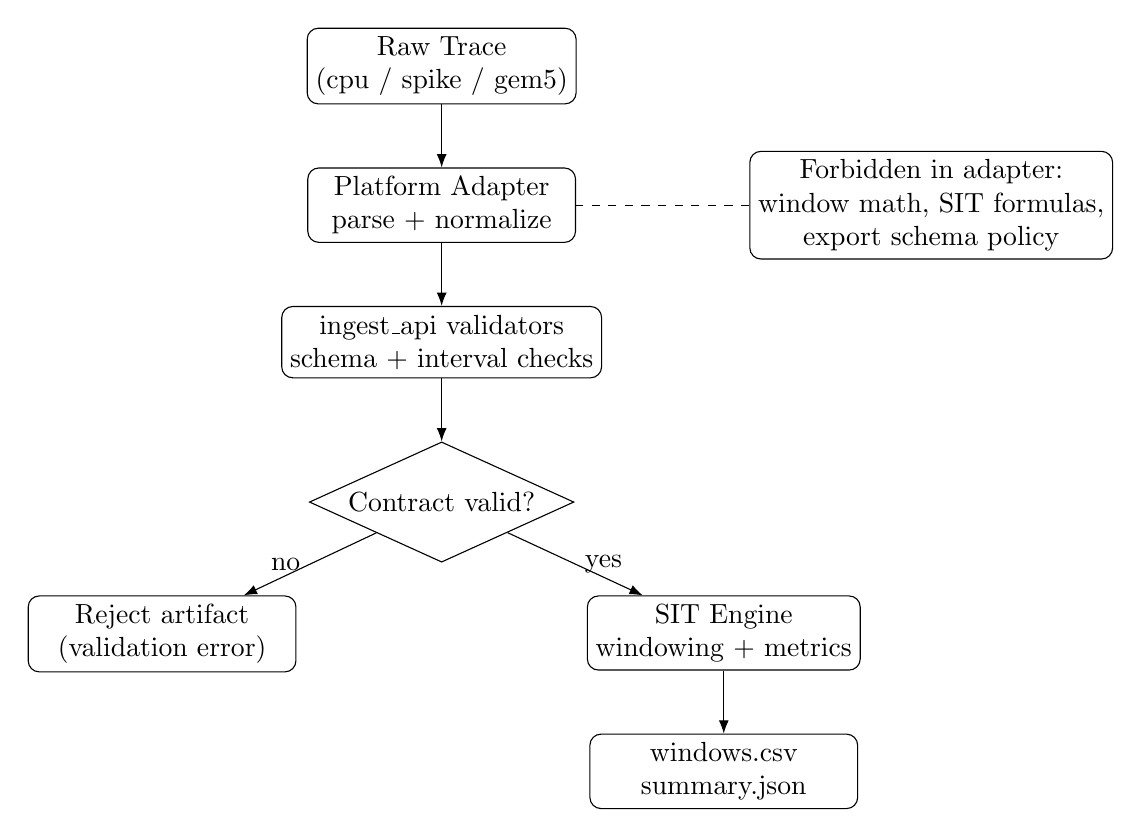
\begin{tikzpicture}[
  node distance=8mm and 10mm,
  box/.style={rectangle, draw, rounded corners, align=center, inner sep=3pt, minimum width=34mm},
  decision/.style={diamond, draw, aspect=2.2, align=center, inner sep=2pt},
  line/.style={-Latex}
]
\node[box] (input) {Raw Trace\\(cpu / spike / gem5)};
\node[box, below=of input] (adapter) {Platform Adapter\\parse + normalize};
\node[box, below=of adapter] (validate) {ingest\_api validators\\schema + interval checks};
\node[decision, below=of validate] (ok) {Contract valid?};
\node[box, below left=of ok] (reject) {Reject artifact\\(validation error)};
\node[box, below right=of ok] (engine) {SIT Engine\\windowing + metrics};
\node[box, below=of engine] (out) {windows.csv\\summary.json};
\node[box, right=22mm of adapter] (forbidden) {Forbidden in adapter:\\window math, SIT formulas,\\export schema policy};

\draw[line] (input) -- (adapter);
\draw[line] (adapter) -- (validate);
\draw[line] (validate) -- (ok);
\draw[line] (ok) -- node[left]{no} (reject);
\draw[line] (ok) -- node[right]{yes} (engine);
\draw[line] (engine) -- (out);
\draw[dashed] (forbidden.west) -- (adapter.east);
\end{tikzpicture}
\end{center}

\end{document}
